\section{NS-3 Network Characterisation and Validation}
\label{sec:network_validation}

\subsection{Analytical Signal-Level Validation}

The analytical check compared the received signal power reported by NS-3 with the value predicted by the Friis model. Five confirmed positions covered a separation range of 58.5--113.8~m, with 150,393 packet samples included in the completed analysis. The comparison produced $R^2=0.860$, an RMSE of 0.77~dB and a mean bias of $-0.77$~dB. Figure~\ref{fig:b1_predicted_observed} shows the overall agreement, while Figure~\ref{fig:b1_residuals} presents the remaining error against distance.

\begin{figure}[htbp]
    \centering
    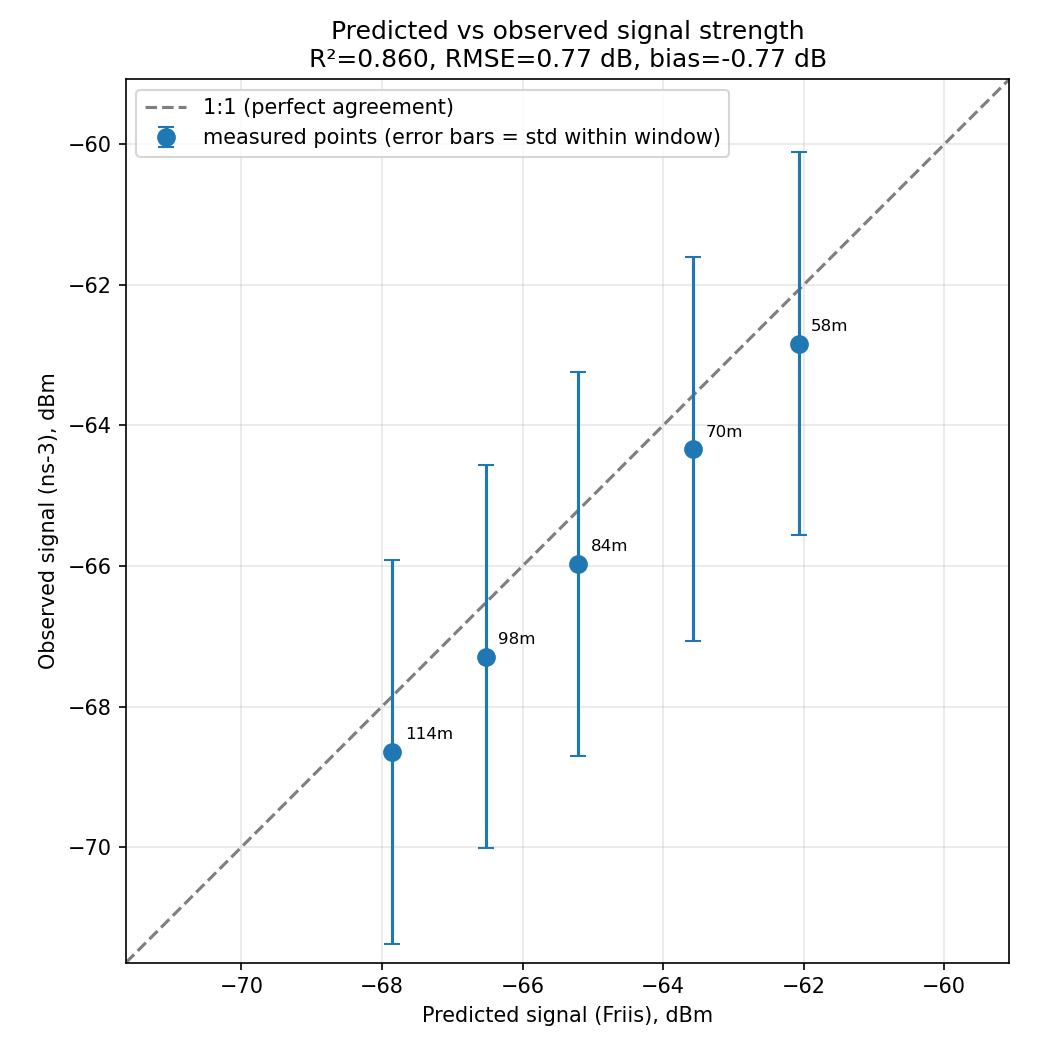
\includegraphics[width=0.76\textwidth]{images/chapter5/network/b1_predicted_vs_observed.png}
    \caption{Friis-predicted and NS-3 observed received signal power at the tested positions.}
    \label{fig:b1_predicted_observed}
\end{figure}

\begin{figure}[htbp]
    \centering
    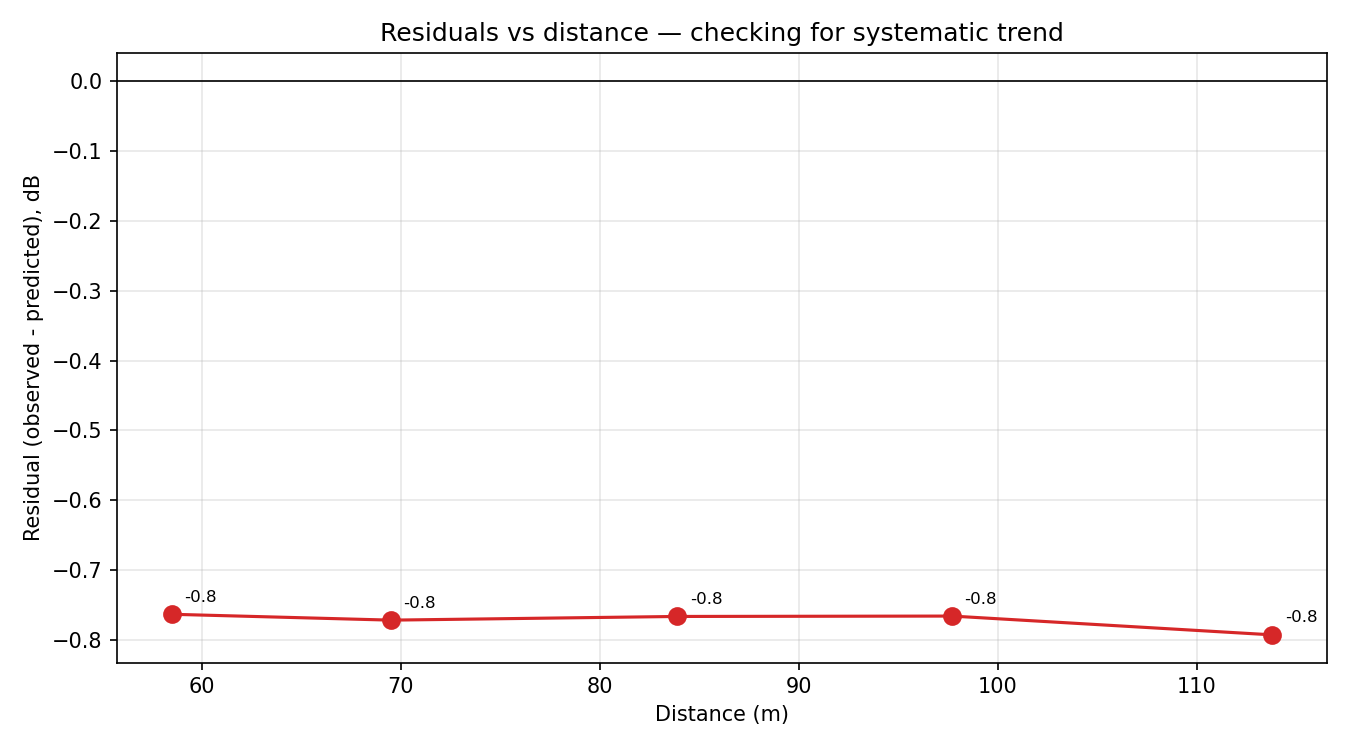
\includegraphics[width=0.82\textwidth]{images/chapter5/network/b1_residuals_vs_distance.png}
    \caption{Difference between the observed and Friis-predicted signal power across distance.}
    \label{fig:b1_residuals}
\end{figure}

The result showed that the simulated signal followed the expected distance-dependent decay reasonably well. A small, almost constant negative offset remained, so the agreement was stronger in the trend than in exact absolute power. This check covered one five-position session and should not be treated as five independent experimental replications.

\subsection{Emulation-Path Timing Characteristics}

Before interpreting RTT against distance, the timing introduced by the test path was checked using the Phase A controls. Table~\ref{tab:phase_a_timing_floor} gives the mean RTT for each condition. The management veth path was close to zero, whereas every NS-3/TAP condition was around 152--161~ms.

\begin{table}[htbp]
    \centering
    \caption{Mean RTT from the Phase A emulation-path controls.}
    \label{tab:phase_a_timing_floor}
    \begin{tabular}{lr}
        \toprule
        Condition & Mean RTT (ms) \\
        \midrule
        Management veth path & 0.032 \\
        Colocated NS-3/TAP path & 158.280 \\
        Operational-distance NS-3/TAP path & 160.700 \\
        Scheduling-control (\texttt{chrt}) & 152.310 \\
        \bottomrule
    \end{tabular}
\end{table}

These values describe an emulation-path timing characteristic. The tests did not isolate its exact internal cause, and the roughly 150~ms floor should not be read as wireless propagation delay.

The B2 and B3 aggregate results were preserved in the project experiment manifest, although their detailed run-level logs were not retained separately.

Table~\ref{tab:b2_rtt_distance} and Figure~\ref{fig:b2_rtt_distance} summarise the B2 RTT measurements. Mean RTT stayed between 153.3 and 159.9~ms, and no packet loss was reported at any of the five positions.

\begin{table}[htbp]
    \centering
    \caption{B2 RTT measurements across the tested UAV separations.}
    \label{tab:b2_rtt_distance}
    \begin{tabular}{rrrrr}
        \toprule
        Distance (m) & Mean (ms) & Minimum (ms) & Maximum (ms) & Loss (\%) \\
        \midrule
        58.5 & 159.8 & 129 & 197 & 0 \\
        69.5 & 153.3 & 119 & 185 & 0 \\
        83.9 & 159.4 & 130 & 194 & 0 \\
        97.7 & 159.9 & 135 & 204 & 0 \\
        113.8 & 158.1 & 127 & 212 & 0 \\
        \bottomrule
    \end{tabular}
\end{table}

\begin{figure}[htbp]
    \centering
    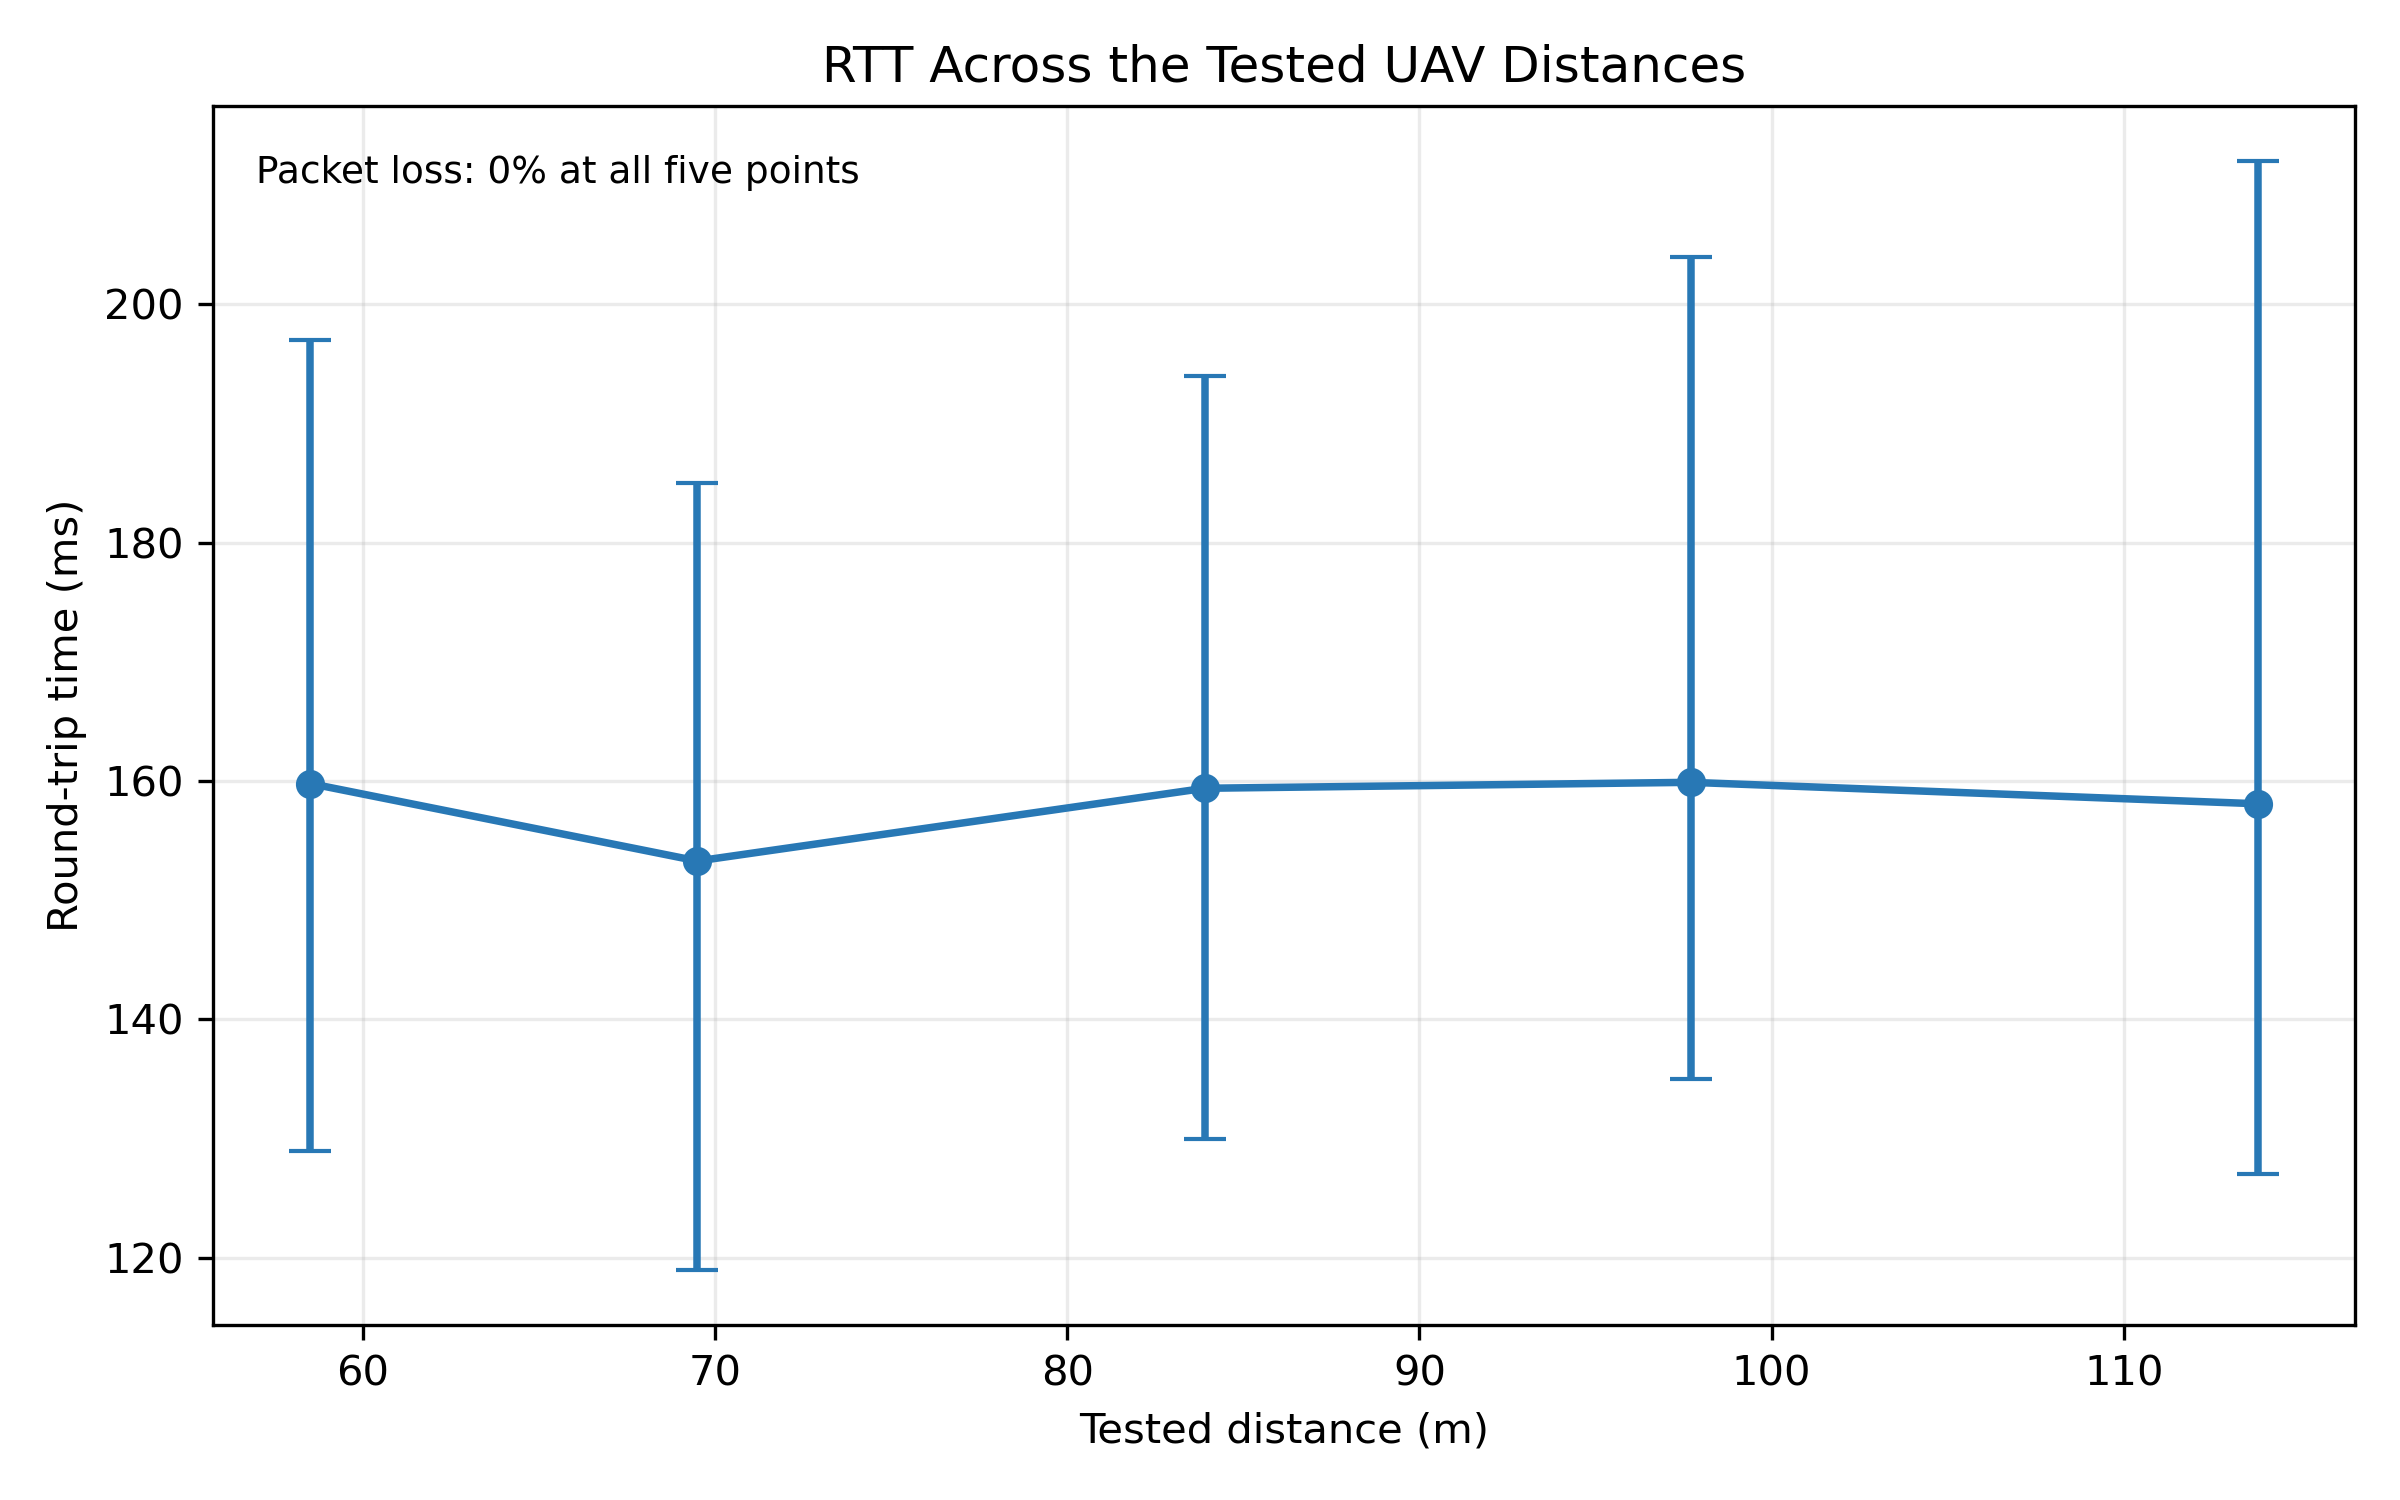
\includegraphics[width=0.82\textwidth]{images/chapter5/network/b2_rtt_vs_distance.png}
    \caption{Mean B2 RTT with the observed minimum-to-maximum range; all tested points recorded zero packet loss.}
    \label{fig:b2_rtt_distance}
\end{figure}

There was no clear distance-dependent increase within this range. Compared with the Phase A controls, the change in propagation time over these distances was small enough to be hidden by the much larger NS-3/TAP timing floor. This does not mean that distance can never affect RTT; it only describes the behaviour seen under the tested conditions.

\subsection{Throughput and Packet-Loss Behaviour}

The offered-load test increased input traffic from 2 to 8~Mbps. As shown in Table~\ref{tab:b3_throughput}, received throughput rose from 1.69 to 3.02~Mbps, but packet loss increased much more sharply.

\begin{table}[htbp]
    \centering
    \caption{B3 received throughput and packet loss against offered load.}
    \label{tab:b3_throughput}
    \begin{tabular}{rrr}
        \toprule
        Offered load (Mbps) & Received throughput (Mbps) & Loss (\%) \\
        \midrule
        2 & 1.69 & 11.0 \\
        5 & 2.85 & 40.0 \\
        8 & 3.02 & 59.6 \\
        \bottomrule
    \end{tabular}
\end{table}

\begin{figure}[htbp]
    \centering
    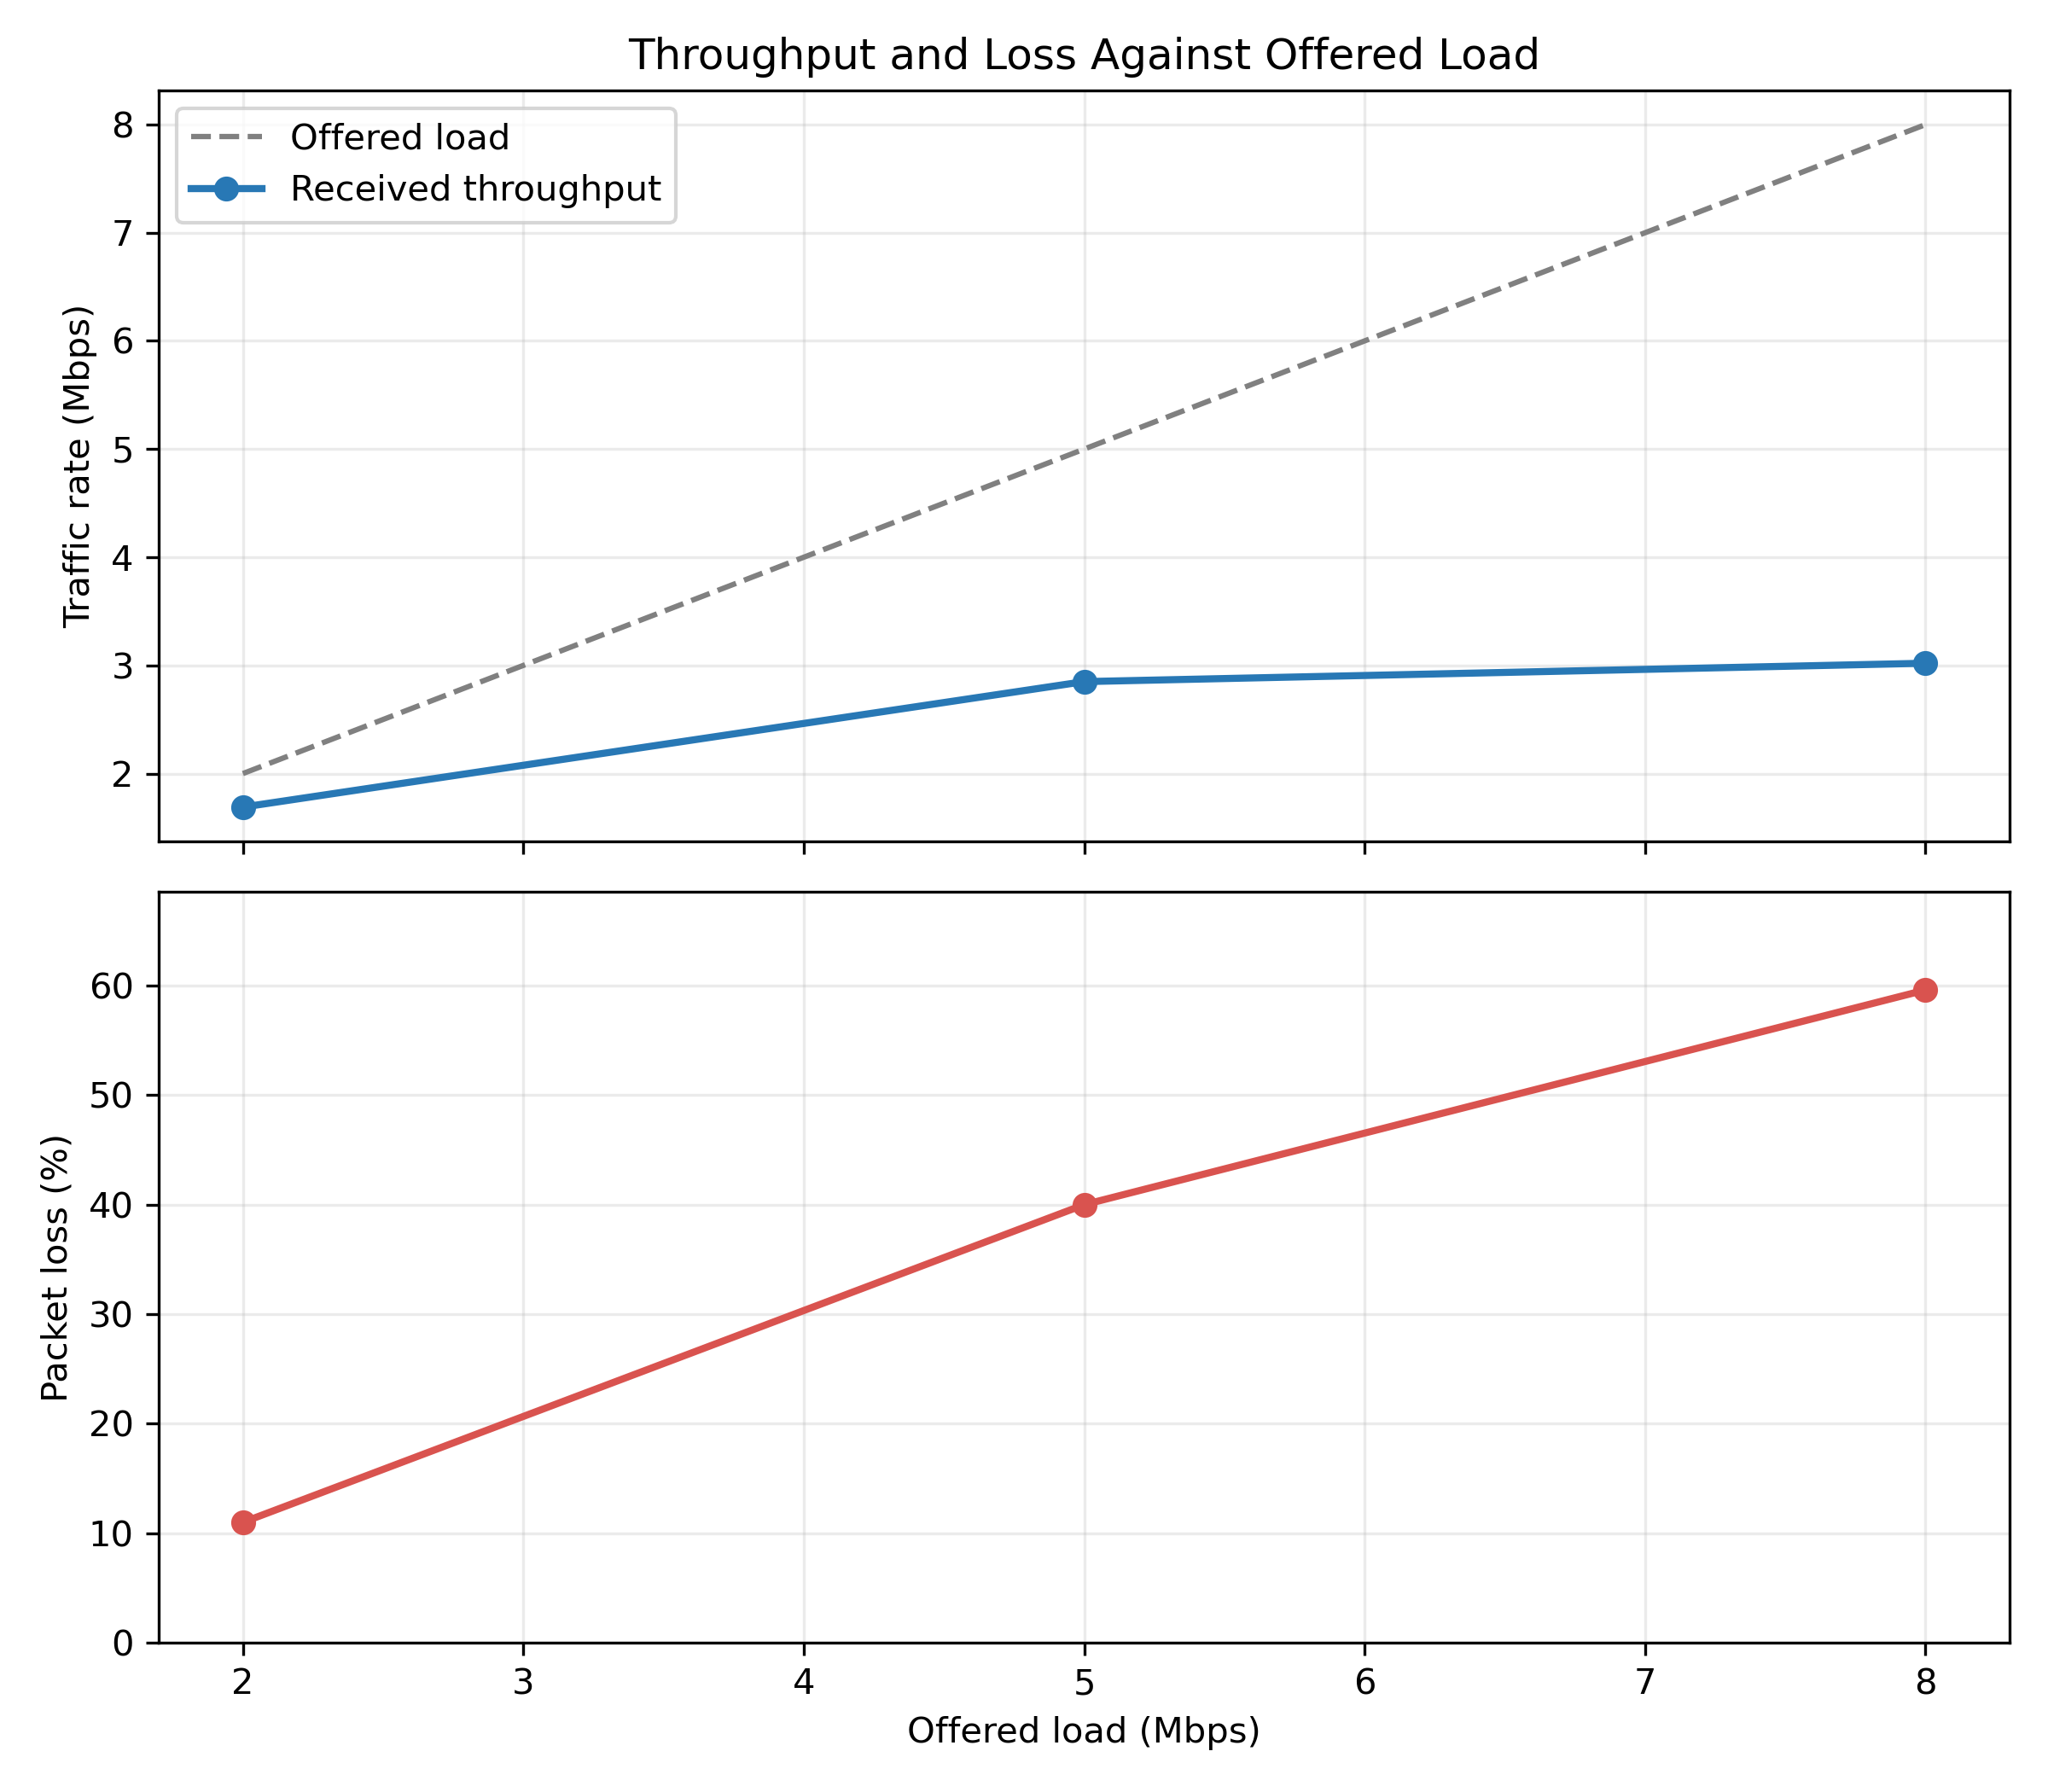
\includegraphics[width=0.82\textwidth]{images/chapter5/network/b3_throughput_and_loss.png}
    \caption{B3 offered load, received throughput and packet loss under the tested configuration.}
    \label{fig:b3_throughput_loss}
\end{figure}

Useful throughput therefore approached a soft ceiling of about 3~Mbps for this setup. Extra offered traffic above that level mainly increased loss. The figure is an observed limit for the selected configuration, rather than a universal capacity of the Wi-Fi standard.

B4 then examined loss at a fixed offered load of 2~Mbps using 10~s runs. Table~\ref{tab:b4_loss_distance} compares the TAP counters with the iperf receiver report. TAP loss remained between 13.25\% and 13.96\%, while iperf reported 11--12\%.

\begin{table}[htbp]
    \centering
    \caption{B4 packet loss across the processed test distances.}
    \label{tab:b4_loss_distance}
    \begin{tabular}{rrr}
        \toprule
        Distance (m) & TAP loss (\%) & iperf loss (\%) \\
        \midrule
        58.50 & 13.96 & 12.00 \\
        69.50 & 13.58 & 11.00 \\
        83.09 & 13.44 & 11.00 \\
        97.70 & 13.25 & 11.00 \\
        113.80 & 13.49 & 11.00 \\
        \bottomrule
    \end{tabular}
\end{table}

\begin{figure}[htbp]
    \centering
    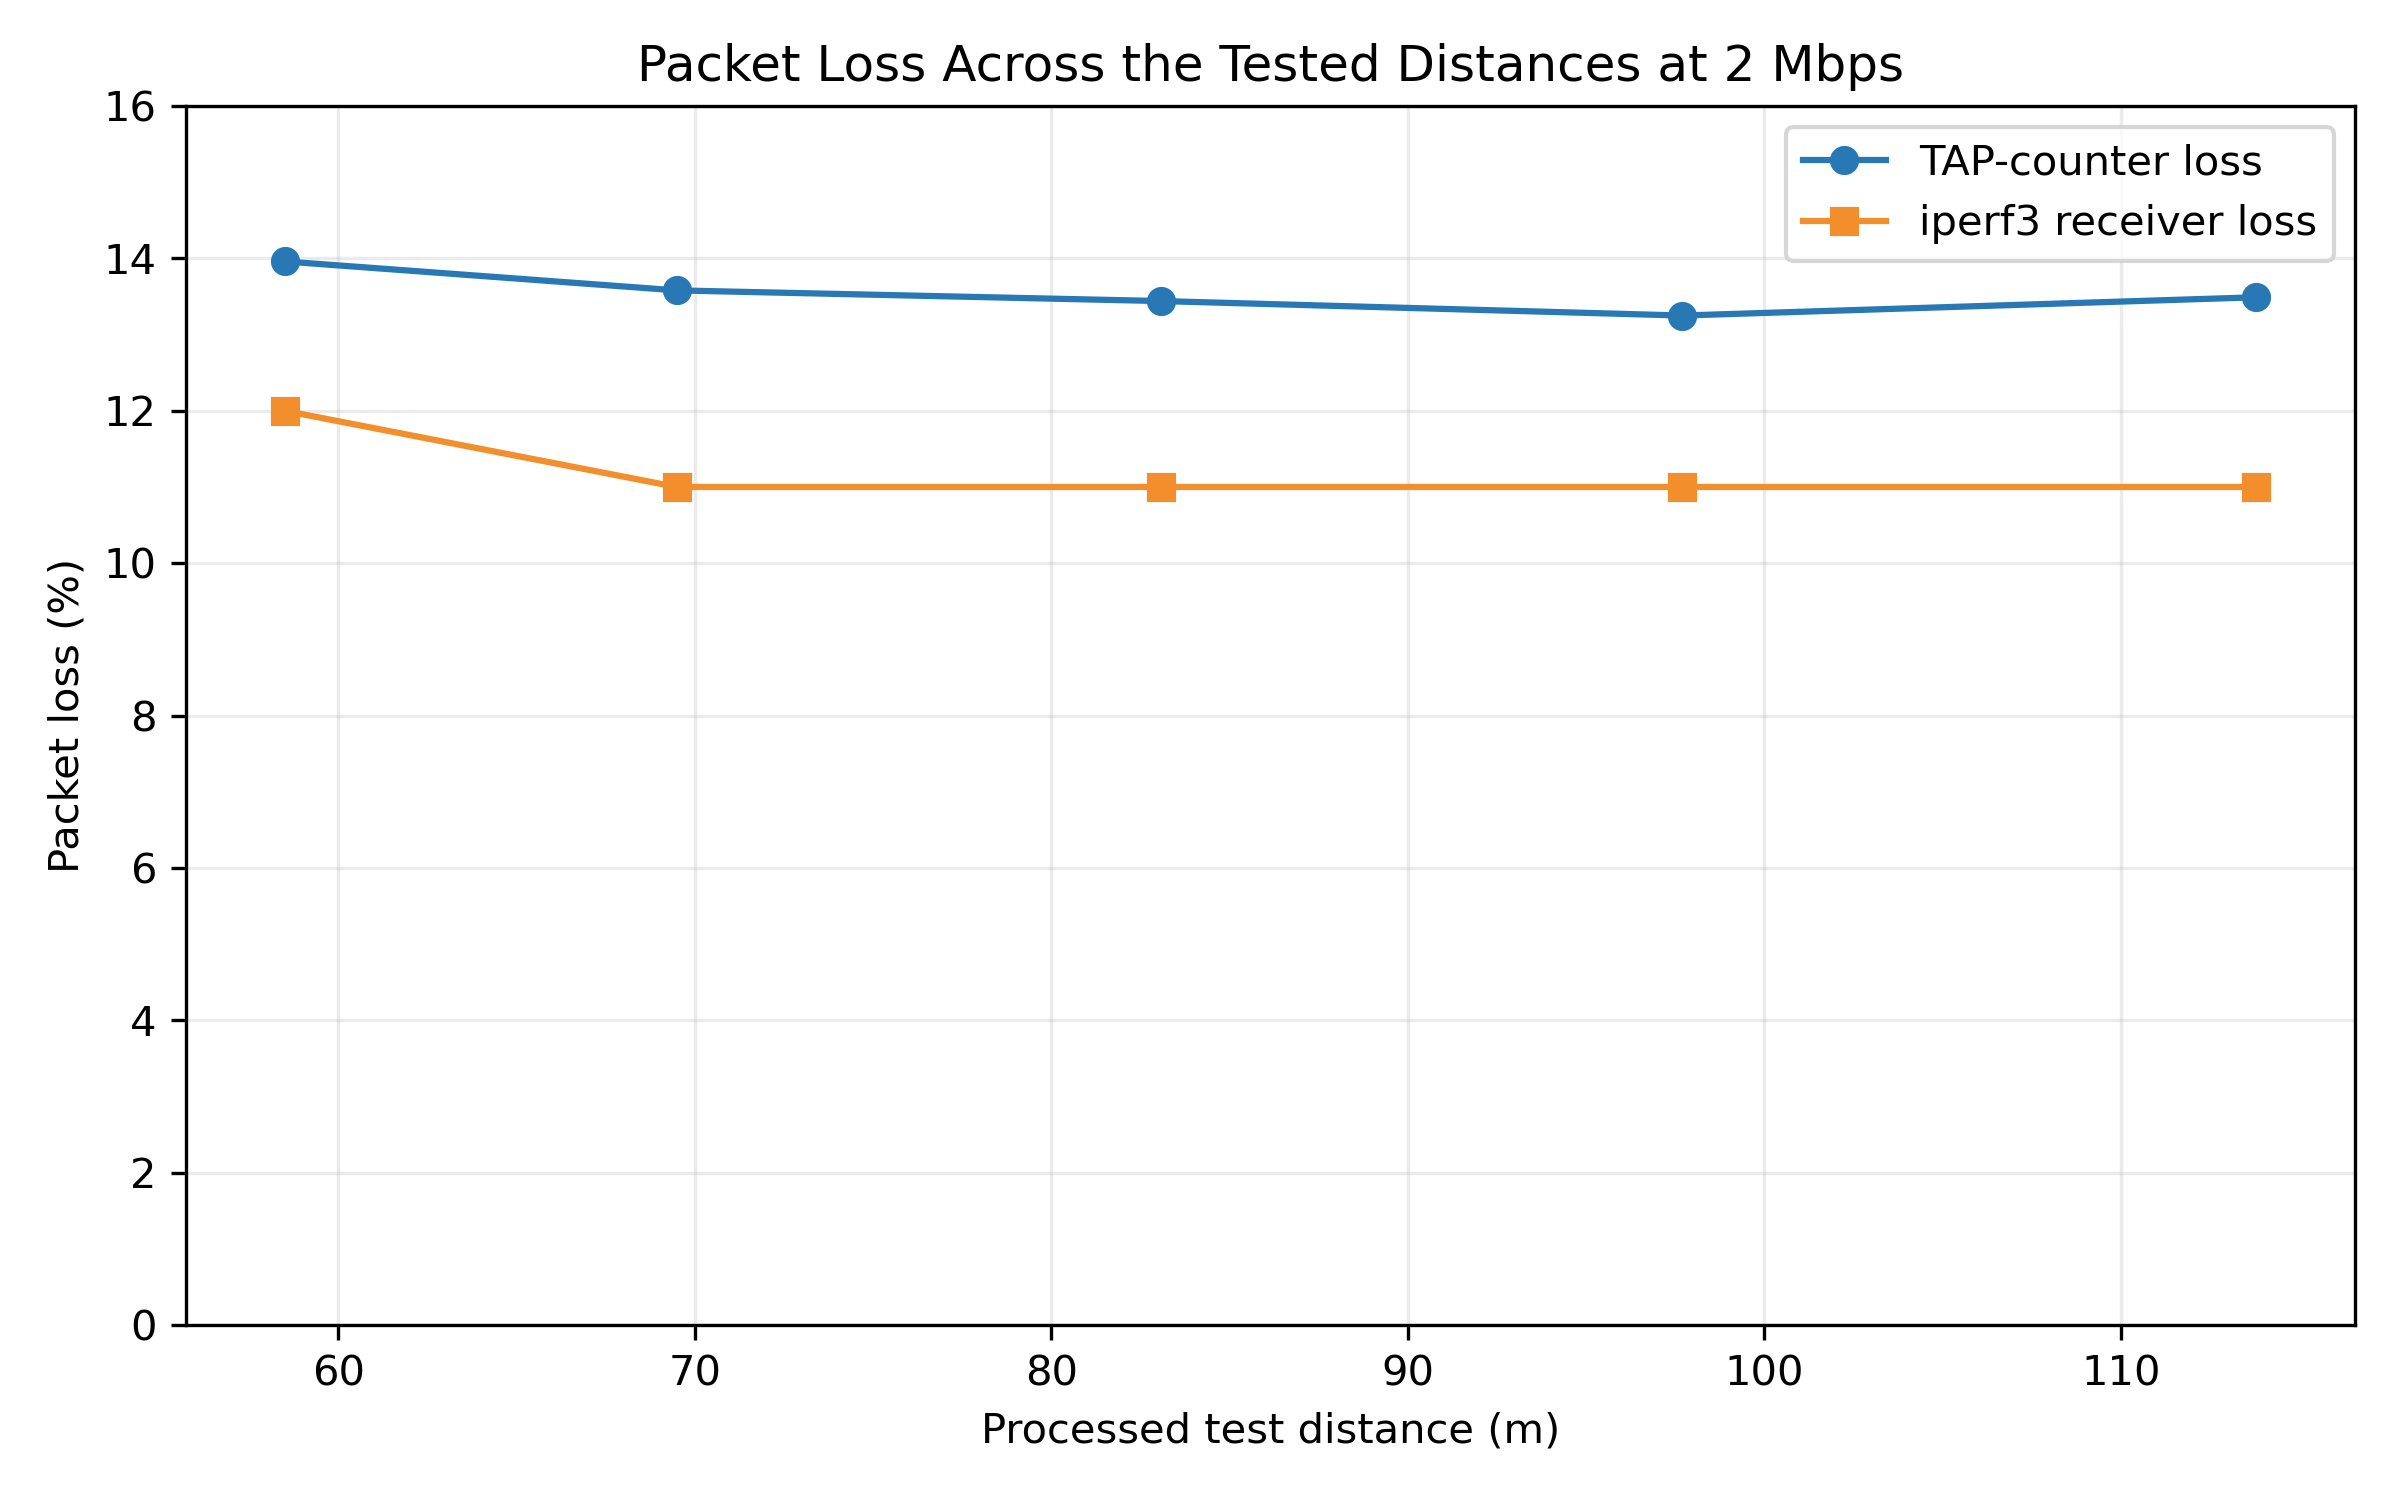
\includegraphics[width=0.82\textwidth]{images/chapter5/network/b4_loss_vs_distance.png}
    \caption{TAP-counter and iperf-reported loss across the B4 distance tests at 2~Mbps.}
    \label{fig:b4_loss_distance}
\end{figure}

Both loss measures stayed broadly similar as distance increased. Within these positions, the traffic load and emulation configuration had a stronger visible effect than the modest change in separation. The finding is limited to the tested range and should not be extended to longer links or different environments without further measurements.

\subsection{Network Validation Summary}

Overall, the signal-level test followed the expected Friis trend, while RTT was mainly shaped by the NS-3/TAP timing floor. Throughput approached roughly 3~Mbps before added load produced substantially more packet loss, and the fixed-load loss test did not show a strong distance trend. Together, these checks support the network model for the tested setup, but they do not establish performance for every distance, environment or UAV swarm size.
